\chapter{Identificación de pines}

La polaridad de los terminales del diodo está especificada en su encapsulado según lo visto en las clases de aula. De todas formas es
posible validar esta polaridad con el multímetro, es justamente lo que se realizará en esta primera actividad

\section{Actividad de laboratorio}

En esta actividad se midió la continuidad de dos diodos 1N4007 (de silicio) y dos diodos 1N60 (de germanio), tanto en polarización directa como inversa.
Estas mediciones permitieron identificar el ánodo y el cátodo de cada diodo, además de verificar su correcto funcionamiento.
Los resultados obtenidos se disponen en la siguiente tabla:

\begin{table}[H]
  \centering
  \begin{tabular}{|>{\centering\arraybackslash}m{3cm}|*{4}{>{\centering\arraybackslash}m{2cm}|}}
    \hline
    \textbf{Sentido de las puntas del multímetro} & \multicolumn{2}{c|}{\textbf{Diodo de germanio}} & \multicolumn{2}{c|}{\textbf{Diodo de silicio}} \\
    \cline{2-5}
    & \textbf{D1} & \textbf{D2} & \textbf{D1} & \textbf{D2} \\
    \hline

    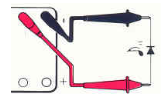
\includegraphics[width=3.2cm]{images/punta1.png} & $355\mV$ & $297\mV$ & $703\mV$ & $620\mV$ \\
    \hline
    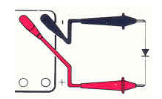
\includegraphics[width=3.2cm]{images/punta2.png} & OL & OL & OL & OL \\
    \hline
  \end{tabular}
  \caption{Mediciones con el multímetro en diferentes polaridades}
\end{table}

\subsection{Imágenes de las mediciones}

\begin{figure}[H]
  \centering
  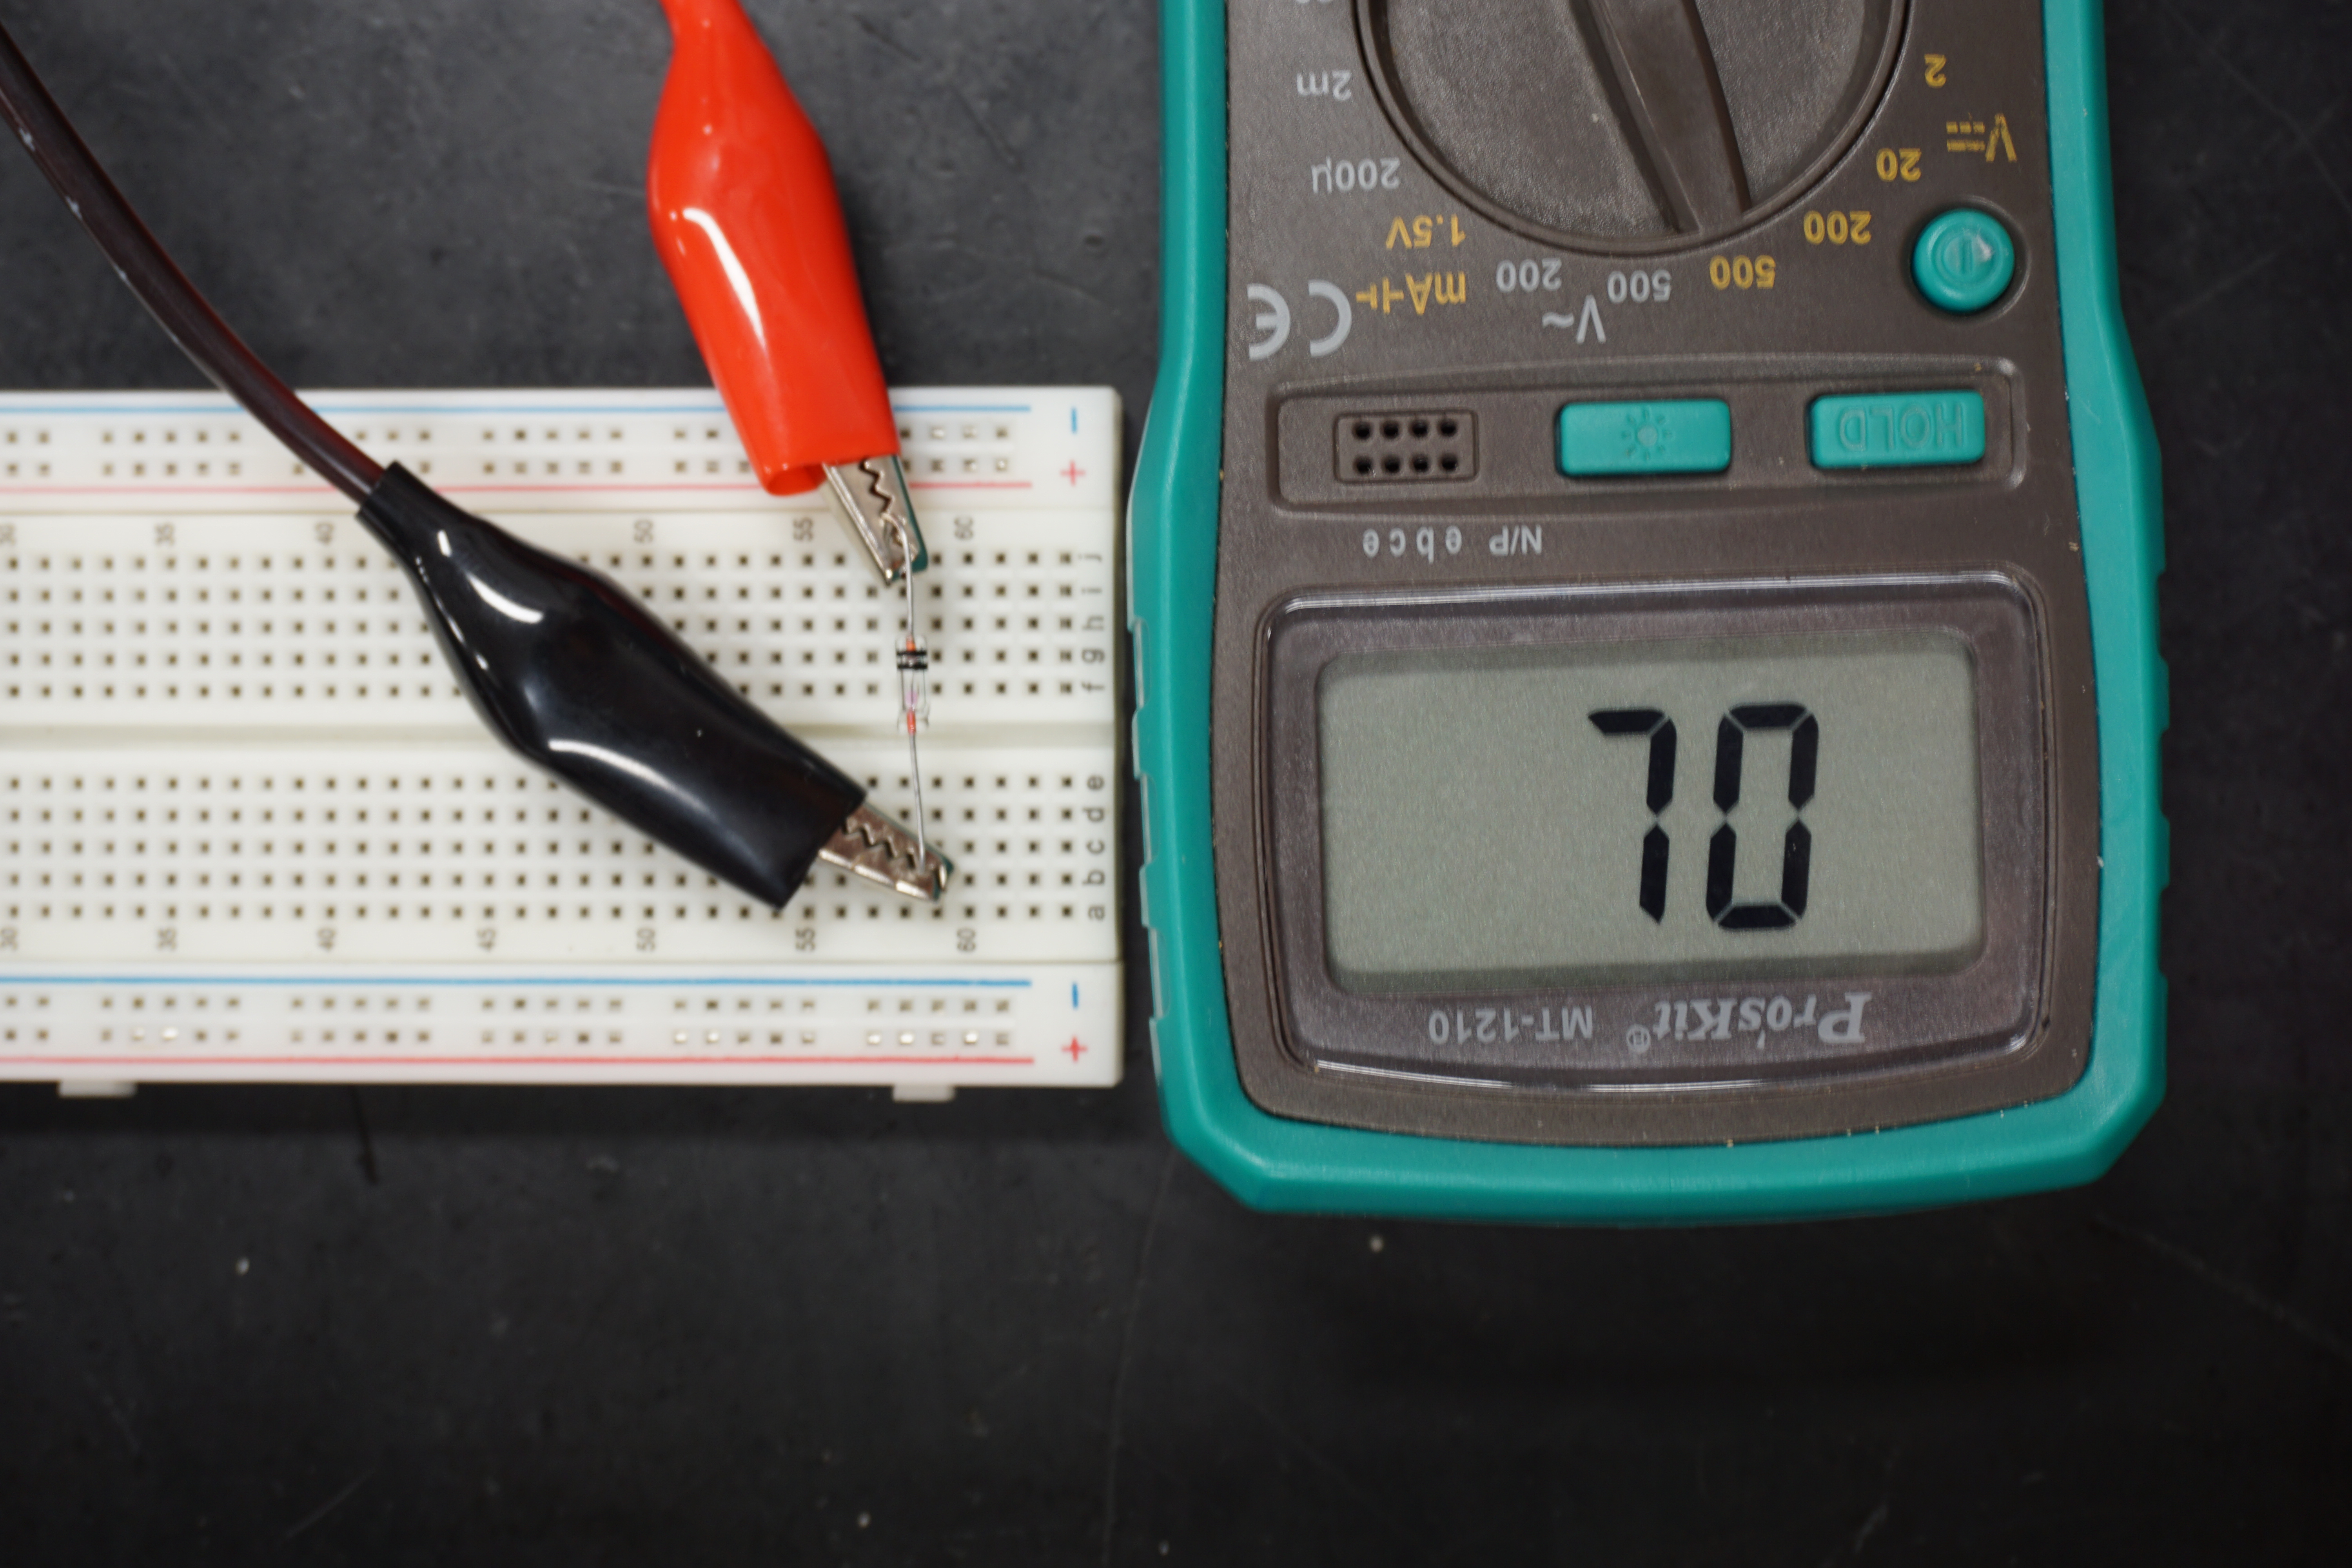
\includegraphics[angle=180, width=0.60\textwidth]{images/diodo1_inversa.png}
  \caption{Diodo de germanio 1 en inversa}
\end{figure}

\begin{figure}[H]
  \centering
  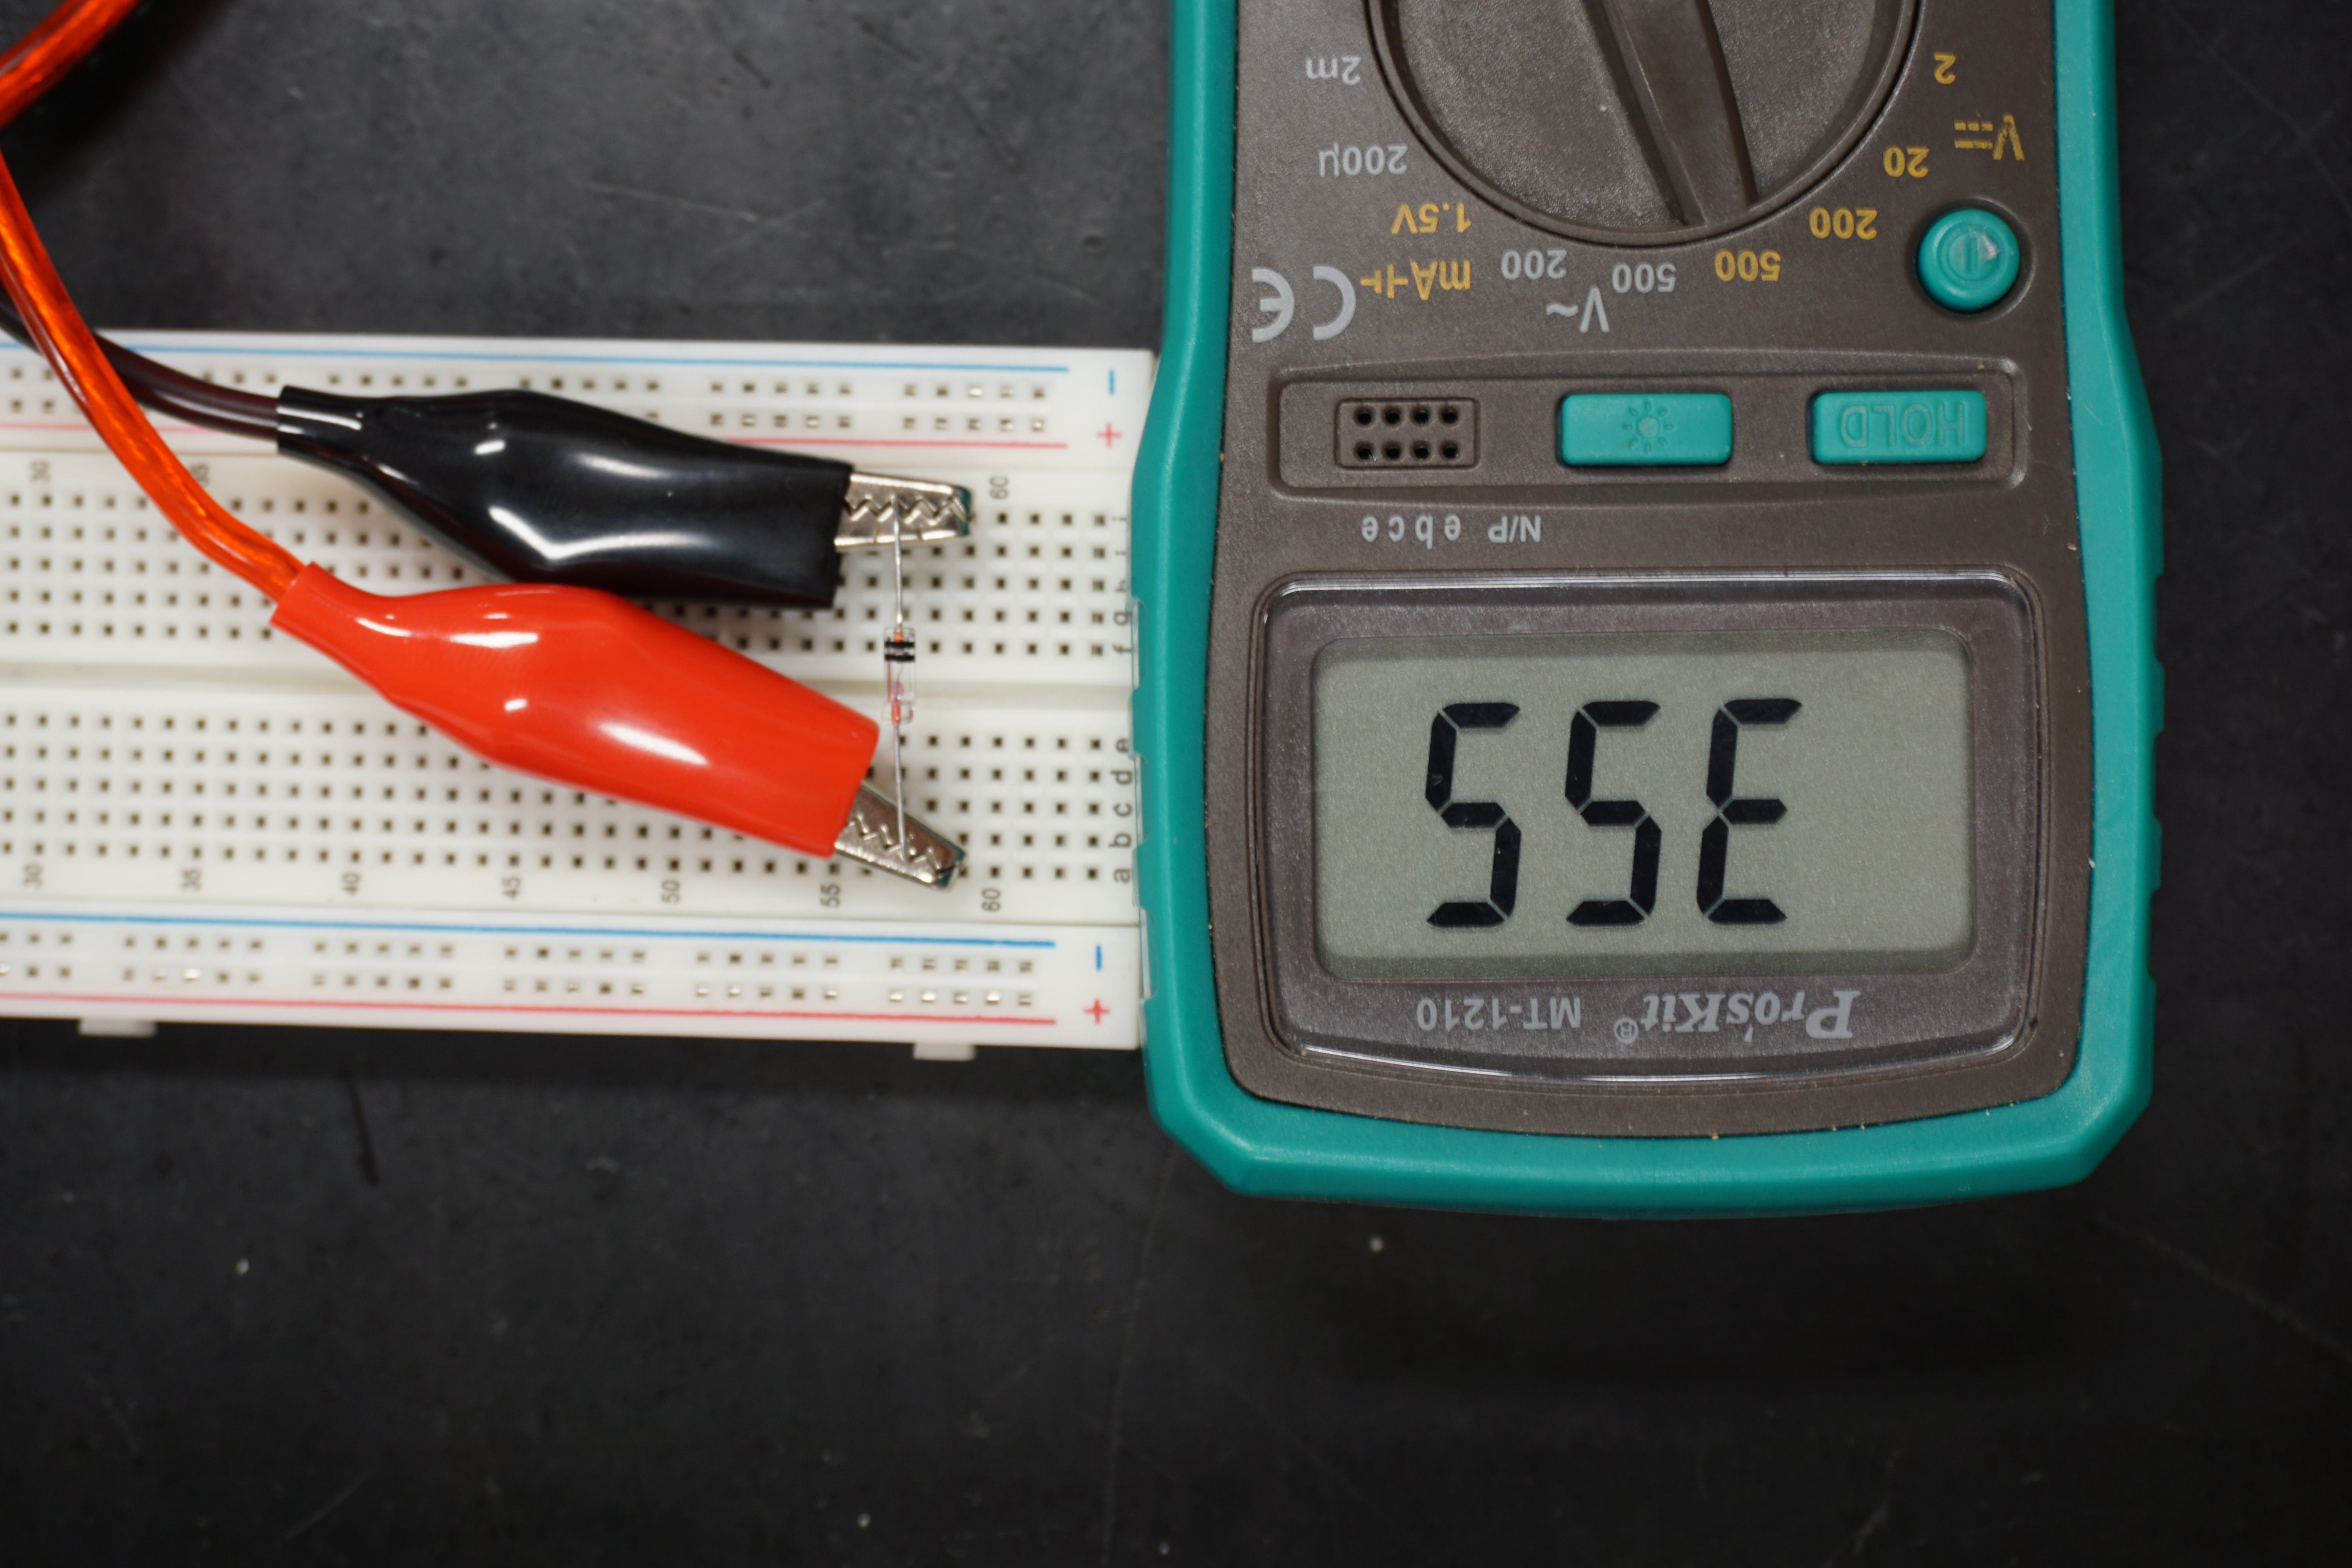
\includegraphics[angle=180, width=0.60\textwidth]{images/diodo1_directa.png}
  \caption{Diodo de germanio 1 en directa}
\end{figure}

\section{Conclusión}

\begin{itemize}
  \item Al medir los diodos utilizando la función de continuidad del multímetro, medimos la caída de tensión de cada diodo.
    En directa, medimos caídas de tensión cercanas a las caídas típicas (0,3V para germanio y 0,7V para silicio).
    En inversa, multímetro nos muestra las siglas OL, de Over Limit en ingles.

  \item Aunque los diodos utilizados eran del mismo tipo, se observaron diferencias en las lecturas. Estas variaciones son normales y pueden
    atribuirse a tolerancias en el proceso de fabricación, diferencias en el dopado de los materiales semiconductores, o a pequeñas
    imperfecciones estructurales internas.

  \item En cada una de las mediciones, los diodos presentaron continuidad en polarización directa, la cual no estuvo presente en polarización inversa, lo que verifica su correcto funcionamiento otorgando parámetros esperables.
\end{itemize}

